%%%%%%%%%%%%%%%%%%%%%%%%%%%%%%%%%%%%%%%%%
% fphw Assignment
% LaTeX Template
% Version 1.0 (27/04/2019)
%
% This template originates from:
% https://www.LaTeXTemplates.com
%
% Authors:
% Class by Felipe Portales-Oliva (f.portales.oliva@gmail.com) with template 
% content and modifications by Vel (vel@LaTeXTemplates.com)
%
% Template (this file) License:
% CC BY-NC-SA 3.0 (http://creativecommons.org/licenses/by-nc-sa/3.0/)
%
%%%%%%%%%%%%%%%%%%%%%%%%%%%%%%%%%%%%%%%%%

%----------------------------------------------------------------------------------------
%	PACKAGES AND OTHER DOCUMENT CONFIGURATIONS
%----------------------------------------------------------------------------------------

\documentclass[
	12pt, % Default font size, values between 10pt-12pt are allowed
	%letterpaper, % Uncomment for US letter paper size
	%spanish, % Uncomment for Spanish
]{fphw}

% Template-specific packages
\usepackage[utf8]{inputenc} % Required for inputting international characters
\usepackage[T1]{fontenc} % Output font encoding for international characters
\usepackage{mathpazo} % Use the Palatino font
\usepackage[dvipsnames]{xcolor}
\usepackage{graphicx} % Required for including images
\usepackage{amsmath}
\usepackage{booktabs} % Required for better horizontal rules in tables
\usepackage{listings} % Required for insertion of code
\usepackage{enumerate} % To modify the enumerate environment
\usepackage{ragged2e}
\usepackage{cancel}
\usepackage{MnSymbol,bbding,pifont}
\usepackage{lscape}
\usepackage{array}
\usepackage{float,graphicx}
\newcolumntype{M}{>{$}c<{$}}
%----------------------------------------------------------------------------------------
%	ASSIGNMENT INFORMATION
%----------------------------------------------------------------------------------------

\title{Assignment \#5} % Assignment title

\author{Luis Alberto Ballado Aradias} % Student name

\date{\today} % Due date

\institute{Centro de Investigación y de Estudios Avanzados del IPN \\ Unidad Tamaulipas} % Institute or school name

\class{Tecnologías Computacionales (Sep - Dec 2022)} % Course or class name

\professor{Dr. Edwin Aldana Bobadilla} % Professor or teacher in charge of the assignment

%----------------------------------------------------------------------------------------

\begin{document}

\maketitle % Output the assignment title, created automatically using the information in the custom commands above

%----------------------------------------------------------------------------------------
%	ASSIGNMENT CONTENT
%----------------------------------------------------------------------------------------

\section*{{\color{Apricot}Memory Allocation}}
%------------------------------------------------

The underlying OS provides some memory to every program that runs and the memory can be divided into two areas.

\begin{itemize}
\item STACK
\item HEAP
\end{itemize}

In every program there are four entities that need to live on this memory

\begin{itemize}
\item Local Variables - Are the variables that are declared inside a method and they live on the stack, they are temporary and they live on the stack as long as the method is executing, so any current executing method along with its local variables lives on the stack until it is done.
\item Methods
\item Objects - Live on the heap and since we know that the instance variables belong to their respective objects instance variables live inside the object on a heap
\item Instance Variables
\end{itemize}

For example:\\

A Car Object (\textbf{Car myCar = new Car();}) which has certain instance variables like: gears, wheels, height. So in heap memory the object always has a sufficient amount of memory to contain all its instance variables. \\

Object creation is a two step process \textbf{Declaration} (\textbf{Car myCar}) and \textbf{Instantiation} (\textbf{new Car();}) \\
In my declaration I have declared a reference variable of the type Car. I have used two keywords here the reference variable and the type car. My Car is called a reference variable, because it does not hold the actual object, just a reference or the address of the memory pointing to the actual object, and car is called a type because car is a class.\\

A class is a logical framework that defines the relationship between it is members, so class is nothing but a user-defined data type and of course I can use this data type to create my reference variable instantiation. The new keyword actually creates the object and the memory is allocated to this object for which the reference is assigned to my Car reference variable, there is one thing that is important here. Since the new keyword allocates memory only at runtime, so the memory gets allocated when the program is executing.\\

\textbf{Constructors} \\

\begin{itemize}
\item Every class has a constructor.
\item A compiler provides the default constructor if no constructor is present in the code.
\item Constructor is called during the lifecycle of an object.
\item Constructor provides a fully initialised usable object immediately upon object creation.
  
\end{itemize}


\section*{{\color{Cerulean}Simple Herence}}
%------------------------------------------------



\section*{{\color{RoyalPurple}Multiple Herence}}
%------------------------------------------------

\begin{figure}[H]
  \centering
  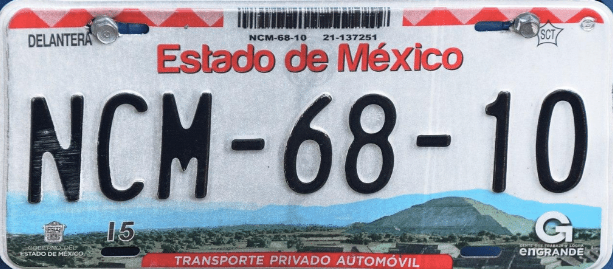
\includegraphics[scale=0.4]{images/placa_auto.png}
\end{figure}


\end{document}
